\documentclass[10pt,a4paper]{article}
% for margining standards
\usepackage[left=3cm,right=3cm,top=3cm,bottom=3cm]{geometry}
% for counting references as a section
\usepackage[numbib,notlof,notlot,nottoc]{tocbibind}
% useful packages
\usepackage{
                graphicx, setspace, fontspec, caption,
                subcaption, float, polyglossia, rotating,
                lscape, pdflscape, indentfirst, tocloft,
                multirow, mathtools, currfile, listings,
                changepage, enumitem, commath
            }
% matlab highlighting package 
\usepackage[framed,numbered,autolinebreaks,useliterate]{mcode}
% paragraph related package
\usepackage[parfill]{parskip}
% use bzar font(THIS MUST BE LOADED BEFORE XePerian PACKAGE)
\setmainfont{BZar.ttf}
% the dear XePersian package
\usepackage{xepersian}
%
% General settings goes here.
%
% lines space
\renewcommand{\baselinestretch}{1.5}
% paragraph first line indention
\setlength{\parindent}{1cm}
% paragraph spacing
\setlength{\parskip}{1em}
% set graphics' path
\graphicspath{ {images/} }
% make table of content dotted
\renewcommand{\cftsecleader}{\cftdotfill{\cftdotsep}}
% define a new command as {half-space} in english
\newcommand{\halfspace}{\hspace{0pt}}
% define a new command as {half-space} in persian
\newcommand{\نیمفاصله}{\halfspace}
% define a shortcut for half-space in general
\renewcommand{\ }{\halfspace}
% define a new command for ease of use for rendering reference
\newcommand{\renderref}[1] { \begingroup \let\clearpage\relax \include{#1} \endgroup }
% shortcut for latin & matlab highlighting code
\renewcommand{\m}[1]{\lr{\mcode{#1}}}
\newcommand{\inlineeqno}{\stepcounter{equation}\ (\theequation)}
\makeatletter
\newenvironment{equationate}{%
    \begin{latin}
    \itemize
    \let\orig@item\item
    \def\item{\orig@item[]\refstepcounter{equation}\def\item{\hfill(\theequation)\orig@item[]\refstepcounter{equation}}}
}{%
    \hfill(\theequation)%
    \enditemize
    \end{latin}
}
\makeatother
%
% DOCUMENT BEGIN
%
\begin{document}
\title{
\begin{figure}[H]
    \centering
    
\includegraphics[width=.2\textwidth]{iut}
\end{figure}
گزارش تکلیف پیاده\ سازی آزمایش اول مقاله\\
\lr{Distributed representation of fuzzy rules and its application to pattern classification}}
\author{داریوش حسن\ پور آده}
\date{۹۳۰۸۱۶۴}
\maketitle
\null
\vfill
% make this very first page un-numbered
\thispagestyle{empty}
\setcounter{page}{0}
\newpage
\قسمت{چکیده}
در این مقاله\
\cite{THEPAPER}
سعی براین بوده است که مفهوم نمایش توزیع\ یافته قوانین فازی را ارائه دهد و در ادامه کاربردی از این مفهوم را در مسایل طبقه\ بندی\زیرنویس{\lr{Classification}} ارائه داده است. هدف از انجام این تکلیف اشنایی با مفهوم قوانین فازی در عمل و انجام آزمایش شماره ۱ مقاله و مقایسه نتایج به دست آمده با نتایج ارائه شده در مقاله می\ باشد. در این مقاله ابتدا مروری بر مفاهیم اولیه مطرح شده توسط مقاله می\ پردازیم سپس درمورد ساختار کدهای نوشته شده صبحتی می\ کنیم و سپس نتایج بدست آمده از آزمایش اول مقاله را ارائه می\ دهیم و در نهایت به نتیجه\ گیری و جمع\ بندی می\ رسیم.
\tableofcontents
\newpage
\قسمت{مقدمه}
برای بدست آوردن قوانین فازی برای دسته\ بندی الگوهای عددی شامل دو قسمت می\ شود:\بند
\vspace{0em}
\begin{enumerate}[nolistsep]
    \setlength{\itemindent}{4em}
    \item تقسیم فضای الگوهای آموزشی
    \item ارائه\ ی قوانینی برای هرکدام از این تقسیم\ بندی\ ها
\end{enumerate}
از مسایل مطرح برای استخراج قوانین فازی برای طبقه\ بندی کردن نمونه\ ها تعیین این مهم که سایز هریک از این تقسیم\ بندی\ ها چقدر باشد تا طبقه\ بند کننده با مشکل
\lr{Overfitting} یا \lr{Underfitting}
مواجه نشود؛ می\ باشد. زیرا که اگر سایز تقسیم\ بندی فضای الگوها درشت باشد قوانین تولیدی برای هر ناحیه از دقت پایینی و در نتیجه طبقه\ بند بدست آمده از قدرت کمتری برخوردار خواهد بود. و از سوی دیگر اگر سایز تقسیم\ بندی فضای الگوها کم باشد به علت زیاد شدن زیر-فضاها\
\زیرنویس{\lr{Sub-Space}}
به قوانین استخراج شده افزوده می\ شود و پیچیدگی طبقه\ بند افزایش می\ یابد و همانند اکثر طبقه\ بندها زمانی که طبقه\ بند پیچیده\ تر شود مشکل
\lr{Overfitting}
پیش می\ آید و همچنین در زمانی که تعداد زیر-فضاها زیاد است ممکن است که زیر-فضایی نمونه\ ای دربر نداشته باشد باعث می\ شود برای برخی از نواحی قوانین تولید نشود.\بند
برای حل مشکلات مذکور مقاله دو راه\ حل نام برده است یکی که مبتنی بر میزان چگالی داده\ ها می\ باشد و ایده به این صورت است که در نواحی\ ای که دارای چگالی داده\ ای زیاد(که معیار می\ تواند تعداد داده\ ها یا آنتروپی داده\ ای باشد) هستند را به نواحی بیشتری شکسته شوند و نواحی با چگالی کم به تعداد زیر-فضاهای کمتری تقسیم شوند. راه\ حل دیگر که راه\ حل ارائه شده توسط مقاله می\ باشد این است که نواحی به صورت تقسیم\ بندی فضای الگوها از تقسیم\ بندی درشت به ریز می\ تواند نتایج مطلوبی ارائه دهد زیرا که اگر در تقسیم\ بندی\ های ریز اگر برای نواحی\ ای قوانینی استخراج نشود حتما در تقسیم\ بندی درشت قوانین برای آن ناحیه بدست خواهد آمد.\\
در ادامه به توضیح مختصری از مقاله و سپس به جزییات پیاده\ سازی انجام شده می\ پردازیم.
\قسمت{قوانین فازی و تقسیم\ بندی فضای الگوها}
در این مقاله فضای الگوها را
$[0, 1] \times [0, 1]$
در نظر گرفته است و این فضا را به
$L^2$
زیر-فضا تقسیم کرده است و به و هر بعد را به پارتیشن\ های
$\{A_1^L, A_2^L,\ldots, A_L^L\}$
تقسیم کرده است. حال طبق ایده\ ی این مقاله که تقسیم\ بندی فضای الگوهای از پارتیشن\ های درشت به پارتیشن\ های ریز بود مقدار
$L$ با مقدار $K$
 که مقداری متغییر می\ باشد و به بازه\ ی
$[2, L]$
محدود می\ باشد جایگزین می\ شود و در نتیجه ما قوانینی در به ازای پارتیشن\ های
$\{A_1^2, A_2^2\}, \{A_1^3, A_2^3, A_3^3\}, \ldots, \{A_1^L, A_2^L,\ldots, A_L^L\}$
بدست می\ آوریم که فرمت این قوانین به صورت
\ref{eq:rule_format}
می\ باشد.
\begin{equationate}\footnotesize
    \item If $x_1$ is $A_i^K$ and $x_2$ is $A_j^K$ then $x_p$ belongs to $G_{ij}^K$ with CF = $CF_{ij}$,\hspace{1em}i, j = 2, 3, \ldots, K;\hspace{1em}K = 2, 3, \ldots, L\label{eq:rule_format}
\end{equationate}
\قسمت{طبقه\ بندی الگوها با استقاده از قوانین فازی}
در این قسمت به شرح مختصری از توابع عضویت مورد استفاده در مقاله و روند استخراج قوانین و استنتاج براساس آنها برای نواحی پارتیشن شده می\ پردازیم.
\زیرقسمت{توابع عضویت}
در این مقاله از ۲ نوع تابع عضویت مثلثی و ذوزنقه برای طبقه\ بندی الگوها استفاده شده است که در زیر به شرح و توضیح منطق عضویت هریک از آن\ ها می\ پردازیم.
\زیرزیرقسمت{تابع عضویت مثلثی}
رابطه تابع عضویت مثلثی مورد استفاده در
\ref{eq:tri_mf}
آمده است.
\begin{equation}
    \mu_i^K(x) = \max\{1 - \abs{x - \frac{i - 1}{k - 1}} (k - 1)\}
    \label{eq:tri_mf}
\end{equation}
 همانطور که در شکل
\ref{fig:tri_mf_K3}
نشان داده شده است نتیجه\ ی اجرای تابع عضویت مثلثی رابطه\ ی
\ref{eq:tri_mf}
برای مقادیر
$K = 3, i = 1, 2, 3$
در بازه\ ی
$[0, 1]$
آورده شده است. منطقی که این تابع عضویت ارائه میدهد این است که هر الگویی با یک درجه\ ی عضویت متعلق به \textbf{همه پارتیشن\ ها} می\ باشد حال هرچقدر الگویی نزدیک به مرز پارتشین\ ها باشد با درجه\ ی عضویت نزدیکی متعلق به هردو پارتیشن همسایه می\ باشد.
\begin{figure}[H]
    \centering
    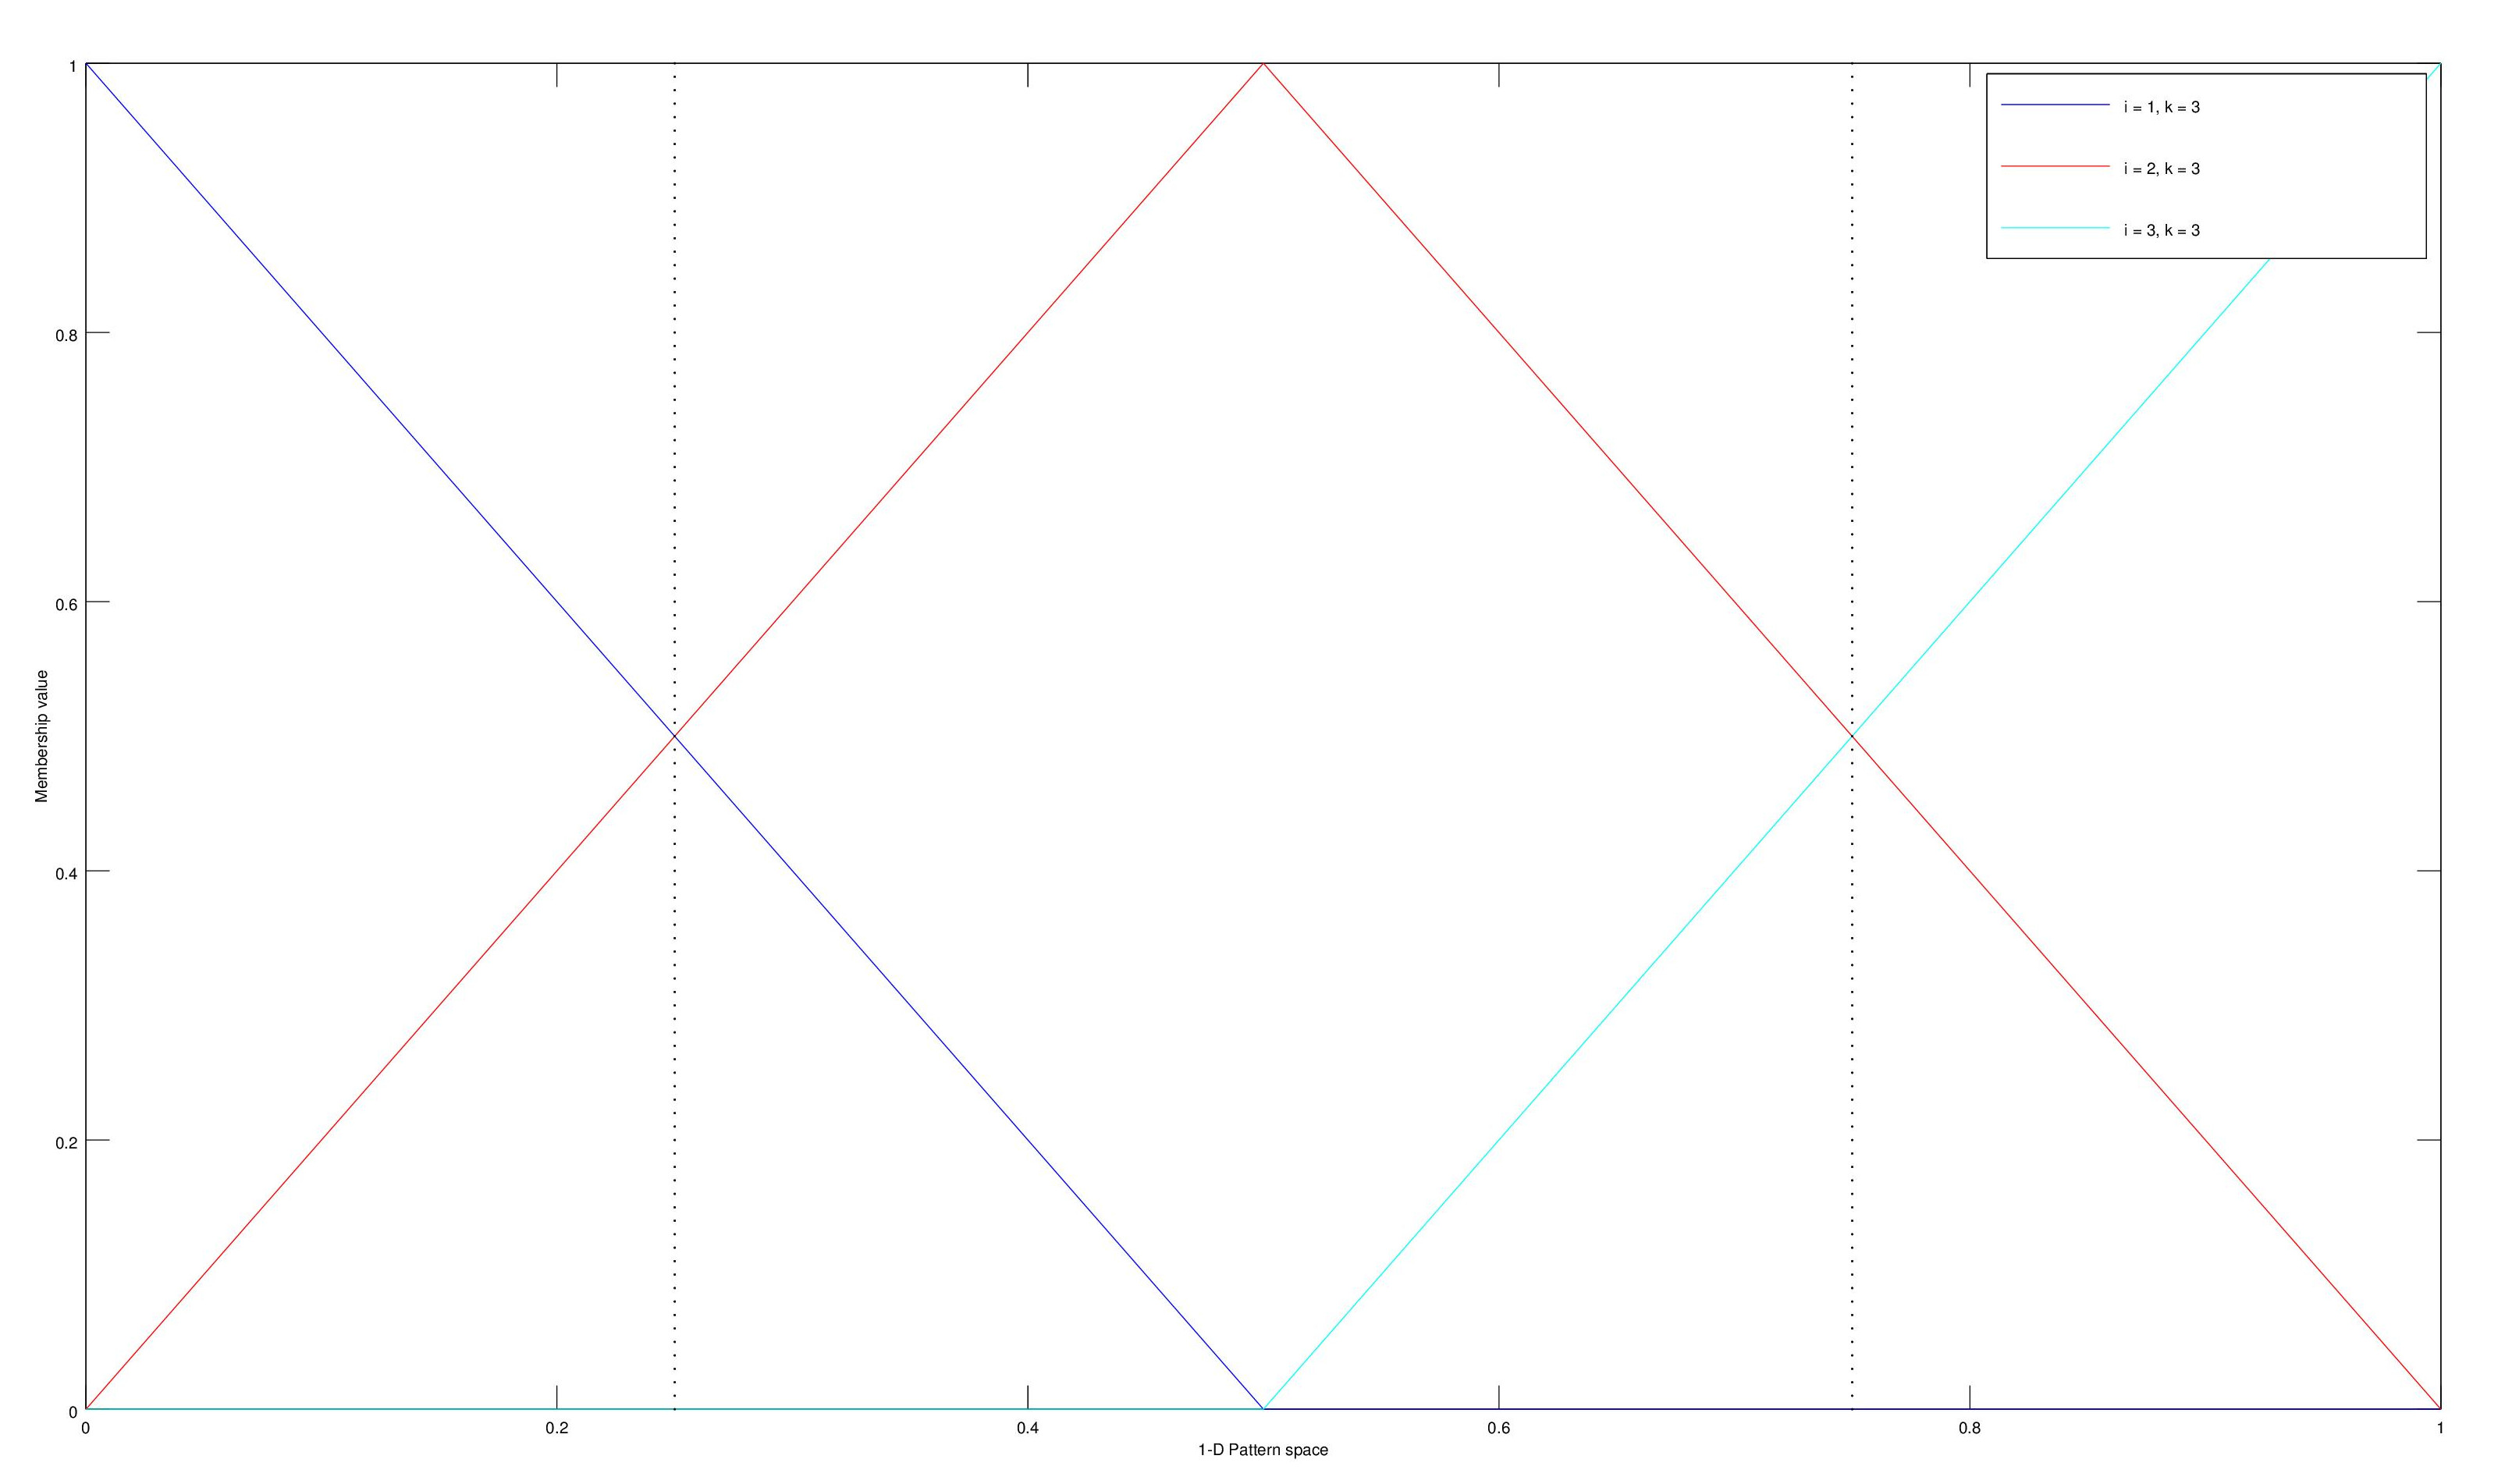
\includegraphics[width=0.9\textwidth]{tri_mf_K3}
    \caption{\small اجرای تابع عضویت مثلثی برای بازه\ ی $[1, 0]$ برای $K = 3$ و $i = 1, 2, 3$}
    \label{fig:tri_mf_K3}
\end{figure}
\زیرزیرقسمت{تابع عضویت ذوزنقه}
رابطه تابع عضویت ذوزنقه مورد استفاده در
\ref{eq:tra_mf}
آمده است.
\begin{equation}
    \mu_i^K(x) = \max\{\min\{2 - 2\abs{x - \frac{i - 1}{k - 1}} (k - 1), 1\}, 0\}
    \label{eq:tra_mf}
\end{equation}
 همانطور که در شکل
\ref{fig:tra_mf_K3}
نشان داده شده است نتیجه\ ی اجرای تابع عضویت ذوزنقه رابطه\ ی
\ref{eq:tra_mf}
برای مقادیر
$K = 3, i = 1, 2, 3$
در بازه\ ی
$[0, 1]$
آورده شده است. منطقی که این تابع عضویت ارائه میدهد این است که هر الگویی با درجه\ ی عضویت ۱ متلق به پارتیشنی که در آن هست می\ باشد و بایک درجه\ ی عضویت متعلق به \textbf{دیگر پارتیشن\ ها} می\ باشد، بطوری که هرچقدر از پارتیشنی که متعلق به آن است دورتر شویم درجه\ ی عضویت آن کاهش می\ باید.
\begin{figure}[H]
    \centering
    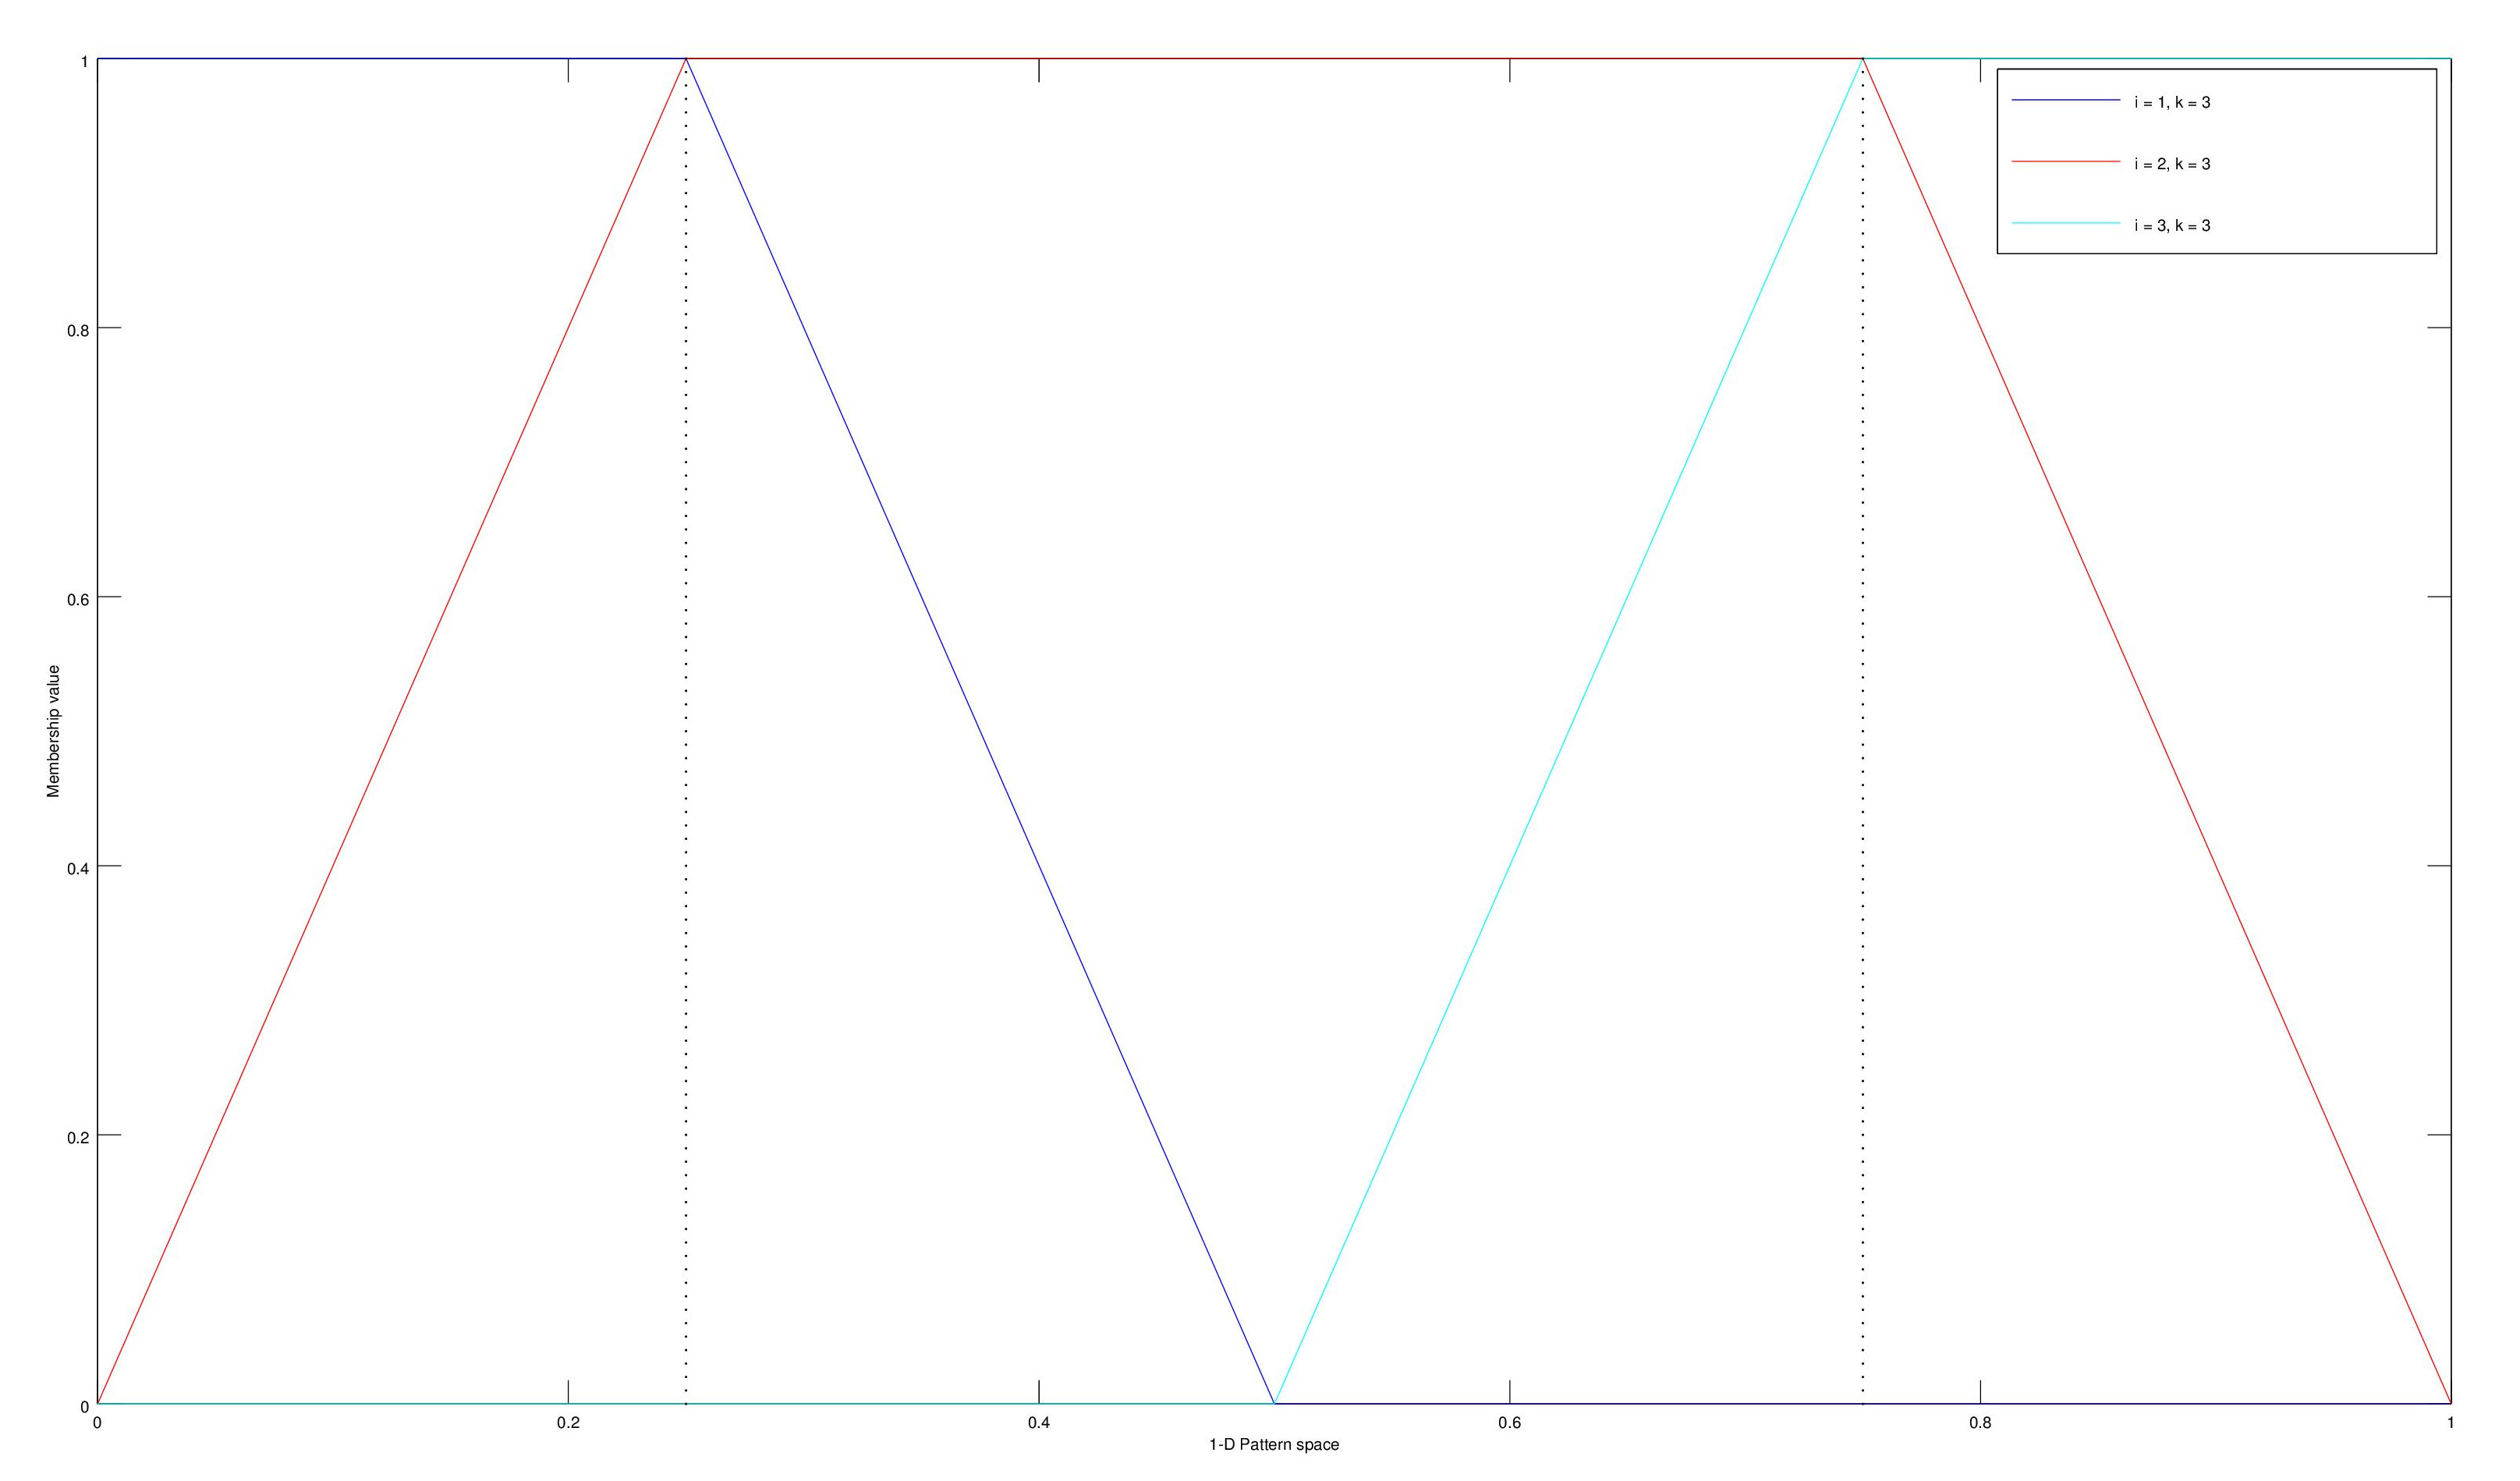
\includegraphics[width=1\textwidth]{tra_mf_K3}
    \caption{\small اجرای تابع عضویت ذوزنقه برای بازه\ ی $[1, 0]$ برای $K = 3$ و $i = 1, 2, 3$}
    \label{fig:tra_mf_K3}
\end{figure}
\زیرقسمت{استخراج قوانین}
\label{sec:rule_extraction}
برای استخراج قوانین به ازای هریک از پارتیشن\ ها میزان سازگاری نمونه\ ها با توجه به درجه\ ی عضویت آن\ ها در آن پارتیشن برای هریک از کلاس\ ها محاسبه می\ کنیم سپس هرکدام از کلاس\ ها که میزان سازگاری بیشتری نسبت به آن پارتیشن را داشت به عنوان برچسب آن پارتیشن با یک درجه\ ی اطمینان درنظر می\ گیریم. میزان سازگاری کلاس\ ها در روابط
\ref{eq:beta_g1_prod} و \ref{eq:beta_g2_prod}
آمده\ اند. همان\ طور که در روابط
\ref{eq:beta_g1_prod} و \ref{eq:beta_g2_prod}
می\ بینیم مقادیر
$\beta_{G1}, \beta_{G2}$
وابسته به داده\ های آموزشی و مقدار $K$ و پارتیشن\ ای که در حال وارسی است($i, j$)، می\ باشد.
\begin{eqnarray}
    \beta_{G1} = \sum_{p \in G1} \mu_i^K(x_{1p}) . \mu_j^K(x_{2p})\label{eq:beta_g1_prod}\\
    \beta_{G2} = \sum_{p \in G2} \mu_i^K(x_{1p}) . \mu_j^K(x_{2p})\label{eq:beta_g2_prod}
\end{eqnarray}
حال بعد از محاسبه\ ی مقادیر
$\beta_{G1}, \beta_{G2}$
به ازای هریک از پارتیشن\ ها پارتیشن\ هایی که مقدار
$\beta_{G1}$
بیشتری نسبت به مقدار
$\beta_{G2}$
دارند به عنوان کلاس
$G1$
برچسب زده می\ شوند و آن پارتیشن\ هایی که مقدار
$\beta_{G2}$
بیشتری نسبت به مقدار
$\beta_{G1}$
دارند به عنوان کلاس
$G2$
برچسب زده می\ شوند. آن پارتیشن\ هایی که مقادیر
$\beta_{G1}$
برابر با
$\beta_{G2}$
می\ باشد را نمی\ توان برچسب دهی کرد. میزان درجه\ ی اطمینان برچسب زده شده به هریک از پارتیشن\ ها نیز وابسته به مقادیر
$\beta_{G1}$
و
$\beta_{G2}$
می\ باشد که در رابطه\ ی
\ref{eq:cf}
آورده شده است.
\begin{equation}
CF_{ij}^K = \frac{\abs{\beta_{G1} - \beta_{G2}}}{\beta_{G1} + \beta_{G2}}
\label{eq:cf}
\end{equation}
در حالت کلی قوانین هر پارتیشن به صورت زیر بدست می\ آید.
\begin{latin}\small
If $x_1p$ is $A_i^K$ and $x_2p$ is $A_j^K$ then $x_p$ belongs to $
\begin{cases}
G1 & \text{if }\beta_{G1} > \beta_{G2} \\
G2 & \text{if }\beta_{G1} < \beta_{G2} \\
Noone & \text{if }\beta_{G1} = \beta_{G2}
\end{cases}$
\hspace{1em}with CF = $CF_{ij}^K$.
\end{latin}
در روابط
\ref{eq:beta_g1_prod} و \ref{eq:beta_g2_prod}
می\ توان از عمگر
$\min$
استفاده کرد که آنگاه روابط
\ref{eq:beta_g1_prod} و \ref{eq:beta_g2_prod}
به صورت روابط
\ref{eq:beta_g1_min} و \ref{eq:beta_g2_min}
خواهند بود.
\begin{eqnarray}
    \beta_{G1} = \sum_{p \in G1} \mu_i^K(x_{1p}) \wedge \mu_j^K(x_{2p})\label{eq:beta_g1_min}\\
    \beta_{G2} = \sum_{p \in G2} \mu_i^K(x_{1p}) \wedge \mu_j^K(x_{2p})\label{eq:beta_g2_min}
\end{eqnarray}
\زیرقسمت{استنتاج و طبقه\ بندی}
بعد از اینکه قوانین فازی که در قسمت
\ref{sec:rule_extraction}
 معرفی شد، استخراج شدند می\ توان با استفاده از قوانین استخراج شده، نمونه\ های جدید برچسب نشده را طبقه بندی کرد. بدین صورت که میزان سازگاری نمونه جدید را با قوانین هریک از کلاس\ ها سنجیده و سپس برچسب نمونه را به کلاسی نسبت می\ دهیم که قوانین حاکم بر آن کلاس دارای بیشترین سازگاری با نمونه را دارند. میزان سازگاری قوانین کلاس\ های
$G1, G2$
به ترتیب در روابط
\ref{eq:alpha_g1_prod} و \ref{eq:alpha_g2_prod}
آمده است.
\begin{eqnarray}
    \alpha_{G1} = \max\{\mu_i^K(x_{1p}) . \mu_j^K(x_{2p}) . CF_{ij}^K \mid G_{ij}^K = G1; \hspace{1em} i, j = 1, 2, \ldots , K;\hspace{1em}K = 2, 3, \ldots , L\}   \label{eq:alpha_g1_prod}\\
    \alpha_{G2} = \max\{\mu_i^K(x_{1p}) . \mu_j^K(x_{2p}) . CF_{ij}^K \mid G_{ij}^K = G2; \hspace{1em} i, j = 1, 2, \ldots , K;\hspace{1em}K = 2, 3, \ldots , L\}   \label{eq:alpha_g2_prod}
\end{eqnarray}
همان\ طور که در روابط
\ref{eq:alpha_g1_prod} و \ref{eq:alpha_g2_prod}
می\ بینیم درجه\ ی اطمینان بدست آمده از بخش استخراج قوانین در محاسبه\ ی میزان سازگاری نمونه با قوانین استفاده شده است و قانونی با بیشترین درجه\ ی اطمینان نقش بیشتری بر میزان سازگاری یک نمونه نسبت به بقیه بازی می\ کند.\بند
بعد از اینکه مقادیر
$\alpha_{G1}, \alpha_{G2}$
را بدست آوردیم، نمونه با یک درجه\ ی اطمینان متعلق به کلاسی است که مقدار
$\alpha$
از دیگری بیشتر است. میزان درجه\ ی اعتبار یا اطمینان طبقه\ بند نیز وابسته به مقادیر
$\alpha_{G_i}$
می\ باشد. بطوری که هرقدر میزان سازگاری قوانین کلاس\ ها با یک نمونه دارای اختلاف بیشتری باشند، با اطمینان بیشتری می\ توانیم طبقه\ بندی کنیم. به عبارت دیگر:
\begin{latin}\small
The new unseen input $x_p$ belongs to $
\begin{cases}
G1 & \text{if }\alpha_{G1} > \alpha_{G2} \\
G2 & \text{if }\alpha_{G1} < \alpha_{G2} \\
Noone & \text{if }\alpha_{G1} = \alpha_{G2}
\end{cases}$
\hspace{1em}with grade of support $\abs{\alpha_{G1} - \alpha_{G2}}$.
\end{latin}
برای زمانی که برای استخراج قوانین از عمگر
$\min$
استفاده شده باشد باید برای محاسبه\ ی روابط
\ref{eq:alpha_g1_prod} و \ref{eq:alpha_g2_prod}
که عمگر ضرب استفاده شده بود از عمگر کمینه استفاده شود. در این صورت باید از روابط
\ref{eq:alpha_g1_min} و \ref{eq:alpha_g2_min}
بجای
\ref{eq:alpha_g1_prod} و \ref{eq:alpha_g2_prod}
استفاده کنیم.
\begin{eqnarray}\tiny
    \alpha_{G1} = \max\{[\mu_i^K(x_{1p}) \wedge \mu_j^K(x_{2p})] . CF_{ij}^K \mid G_{ij}^K = G1; \hspace{1em} i, j = 1, 2, \ldots , K;\hspace{1em}K = 2, 3, \ldots , L\}   \label{eq:alpha_g1_min}\\\tiny
    \alpha_{G2} = \max\{[\mu_i^K(x_{1p}) \wedge \mu_j^K(x_{2p})] . CF_{ij}^K \mid G_{ij}^K = G2; \hspace{1em} i, j = 1, 2, \ldots , K;\hspace{1em}K = 2, 3, \ldots , L\}   \label{eq:alpha_g2_min}
\end{eqnarray}
نحوه\ ی استنتاج از مقادیر روابط
\ref{eq:alpha_g1_min} و \ref{eq:alpha_g2_min}
همانند روند استنتاجی که در مورد روابط
\ref{eq:alpha_g1_prod} و \ref{eq:alpha_g2_prod}
معرفی شد می\ باشد.
\newpage
\قسمت{پیاده\ سازی مقاله}
در پیاده\ سازی انجام شده توابع در حالت کلی به ۳ دسته تقسیم می\ شوند -- قسمتی برای استخراج قوانین فازی و قسمتی برای استنتاج از قوانین بدست آمده در بخش قبل و دسته\ ای از توابع ابزاری\زیرنویس{\lr{Utility Functions}} که در هر دوقسمت قبلی مورد استفاده قرار می\ گیرند. که هریک از این بخش\ ها به ترتیب در زیر توضیح داده می\ شود.
\زیرقسمت{استخراج قوانین}
\زیرزیرقسمت{تابع استخراج قوانین}
تابع \lr{gen\_rules} تنها تابعی که برای استخراج قوانین مورد استفاده قرار می\ گیرد تابع
\m{gen_rules(.)}
می\ باشد. که این تابع ۷ عدد ورودی می\ گیرد که در جدول
\ref{tab:gen_rules}
شرح داده شده\ اند.
\begin{latin}
    \begin{table}[h]
        \centering
        \begin{tabular}{ | l | l | l | }
            \hline        
            Argument   & Type         & Comment\\\hline
            l\_max     & Integer      & The maximum L value to partion the patterns' space\\\hline
            x1         & float        & The patterns' first demintions' value\\\hline
            x2         & float        & The patterns' first demintions' value\\\hline
            func       & function     & The classify function(The problems 1{\ldots}7)\\\hline
            mf\_func   & function     & The membership function(triangular or trapezoid)\\\hline
            mf\_opt    & function     & The operation function for membership-values arithmetic(product or min)\\\hline
            apply\_cf  & boolean      & Indicator that if applying CF is in effect or not?(true or false)\\\hline
        \end{tabular}
        \caption{\mcode{function rules = gen_rules(l_max, x1, x2, func, mf_func, mf_opr, apply_cf)}}
        \label{tab:gen_rules}
    \end{table}
\end{latin}
خروجی تابع
\m{function rules = gen_rules(.)}
یک ماتریسی عددی\زیرنویس{\lr{Numerical}} از قوانین است که فرمت هر قانون این ماتریس به صورت
\m{[k i j g cf]}
می\ باشد که شرح هرکدام از المان\ های قانون در جدول
\ref{tab:gen_rule_return}
آمده است.
\begin{latin}
    \begin{table}[h]
        \centering
        \begin{tabular}{ | l | l | l | }
            \hline        
            Label    & Type       & Comment\\\hline
            k        & integer    & The $K$ value that rule has been generated within\\\hline
            i        & integer    & The region number in first dimension\\\hline
            j        & integer    & The region number in second dimension\\\hline
            g        & [1 or 2]   & The class number\\\hline
            cf       & float      & The confidence level of rule\\\hline
        \end{tabular}
        \caption{Description of generated rule's format}
        \label{tab:gen_rule_return}
    \end{table}
\end{latin}
\زیرقسمت{استنتاج از قوانین}
\زیرزیرقسمت{تابع استنتاج از قوانین و طبقه\ بند}
تابع \lr{classifier} تنها تابعی که مسئولیت طبقه\ بندی داده\ ها را دارد این تابع می\ باشد و دارای ۵ عدد ورودی می\ باشد که در جدول
\ref{tab:classifier}
شرح داده شده\ اند.
\begin{latin}
    \begin{table}[h]
        \centering
        \begin{tabular}{ | l | l | l | }
            \hline        
            Argument   & Type         & Comment\\\hline
            rules      & Integer      & The generated rules\\\hline
            xp         & Matrix       & The un-classified patterns\\\hline
            mf\_func   & function     & The membership function(triangular or trapezoid)\\\hline
            mf\_opt    & function     & The operation function for membership-values arithmetic(product or min)\\\hline
            apply\_cf  & boolean      & Indicator that if applying CF is in effect or not?(true or false)\\\hline
        \end{tabular}
        \caption{\mcode{function z = classifier(rules, xp, mf_func, mf_opr, apply_cf)}}
        \label{tab:classifier}
    \end{table}
\end{latin}
خروجی تابع
\m{function z = classifier(.)}
یک ماتریس کلاسی می\ باشد هر سطر این ماتریس متناظر با یک سطر از ماتریس الگوهای ورودی تابع می\ باشند و فرمت هر سطر به صورت
\m{[g cf]}
می\ باشد که سرح هرکدام از المان\ ها در جدول
\ref{tab:classifier_return}
آمده است.
\begin{latin}
    \begin{table}[h]
        \centering
        \begin{tabular}{ | l | l | l | }
            \hline        
            Label    & Type       & Comment\\\hline
            g        & [1 or 2]   & The class number\\\hline
            cf       & float      & The confidence level of classification\\\hline
        \end{tabular}
        \caption{Description of classification's output's format}
        \label{tab:classifier_return}
    \end{table}
\end{latin}
\زیرقسمت{توابع ابزاری}
توابع ابزاری بیشتر برای کارهای ابتدایی مانند تولید نمونه و توابع عضویت و \ldots\hspace{1pt} می\ باشند که از درجه اهمیت کمتری نسبت به توابع ذکر شده برخور دارند که بجز تابع راه\ انداز\زیرنویس{\lr{Bootstrapper}}\
[\m{frpc(.)}]
فقط به نام\ بردن و ذکر هدف دیگر توابع ابزاری بسنده می\ کنیم.
\begin{latin}
    \begin{table}[h]
        \centering
        \begin{tabular}{ | l | l | p{8cm} | }
            \hline        
            Function                   & Retune Type  & Comment\\\hline
            frpc                       & void         & The bootstrapper (to be explained).\\\hline
            gen\_data                  & Matrix       & Generates random data in $[0, 1]\times[0, 1]$ pattern space with uniform distribution.\\\hline
            value2class                & [1 or 2]     & Converts its input values into 2 class-type [1 or 2].\\\hline
            mf\_trapezoid              & float        & The trapeziod membership function.\\\hline
            mf\_triangular             & float        & The triangular membership function.\\\hline
            print\_rules               & void         & Prints the passed rules in maner of a nice verbal format.\\\hline
            print\_classification\_res & void         & Prints the classification results in maner of a nice verbal format.\\\hline
        \end{tabular}
        \caption{List of utility functions}
        \label{tab:utility_functions}
    \end{table}
\end{latin}
از میان توابع جدول
\ref{tab:utility_functions}
تابع راه\ انداز که وظیفه\ ی راه\ اندازی پروژه و انجام عملیات تولید قوانین فازی و تست قوانین و چاپ نتایج حاصل از تست دارد به عهده دارد نیاز به توضیح بیشتری راجع به فازهای اجرایی خود دارد.\بند
\زیرزیرقسمت{تابع راه\ انداز}
تابع \lr{frpc} به عنوان ورودی یک مقدار
$l_max$
دریافت می\ کند که مقدار پیش\ فرض این ورودی ۱۰ می\ باشد. سپس با یکی از توابع مسائل
۱{\ldots}۷
که در اینجا تابع مساله\ ی ۱ مورد استفاده قرار گرفته شده است. سپس برای انجام آزمایشات یک داده\ ی تست به صورت تصادفی تولید شده است که همه آزمایشات روی یک داده تست انجام شده باشند که تنایج آزمایشات قابل مقایسه با یک دیگر باشند.\بند
طبق جدول ۱ مقاله که از دو تیپ-تعدادی داده\ ی آموزشی برای تولید قوانین استفاده کرده است، که به صورت یک داده\ ی آموزشی ۴۰ تایی و یک داده\ ی آموزشی ۱۰۰ تایی و در هردوی این\ ها تعداد داده\ های تست ۱۰۰ عدد هستند. بدین منظور بنده نیز ۲ دسته ۴۰ تایی  و ۱۰۰ تایی به عنوان داده\ ی آموزشی در داخل یک حلقه تولید میکنم. سپس به ازای هر داده آموزشی ۶ تست مطرح در جدول شماره\ ی ۱ مقاله را در داخل حلقه\ دوم اجرا میکنم که مقادیر متغییر\ های در تست از تابع \m{get_opt} که وابسته به شماره تست(که شماره تست\ ها متناسب با تست\ های جدول ۱ در نظر گرفته شده اند.) می\ باشد. سپس با استفاده از داده آموزشی قوانین فازی استخراج شده و سپس قوانین بروی داده\ ی تست آزموده می\ شود و سپس نتایج تست چاپ می\ شوند.
\قسمت{آزمایش اول}
جدول
\ref{tab:results}
\textbf{میانگین}
مساله\ ی یک مقاله که در رابطه\ ی
\ref{eq:problem_1}
آورده شده است. فضای الگوی
$[0, 1] \times [0, 1]$
را به صورت غیرخطی به دو بخش مثبت و منفی تقسیم می\ کند که در شکل
\ref{fig:problem_1}
آمده است.
\begin{latin}
\begin{equation}
f_1(x) = -\frac{1}{4}\sin{(2{\pi}x_1)} + x_2 - 0.5
\label{eq:problem_1}
\end{equation}
\end{latin}

\begin{figure}[H]
    \centering
    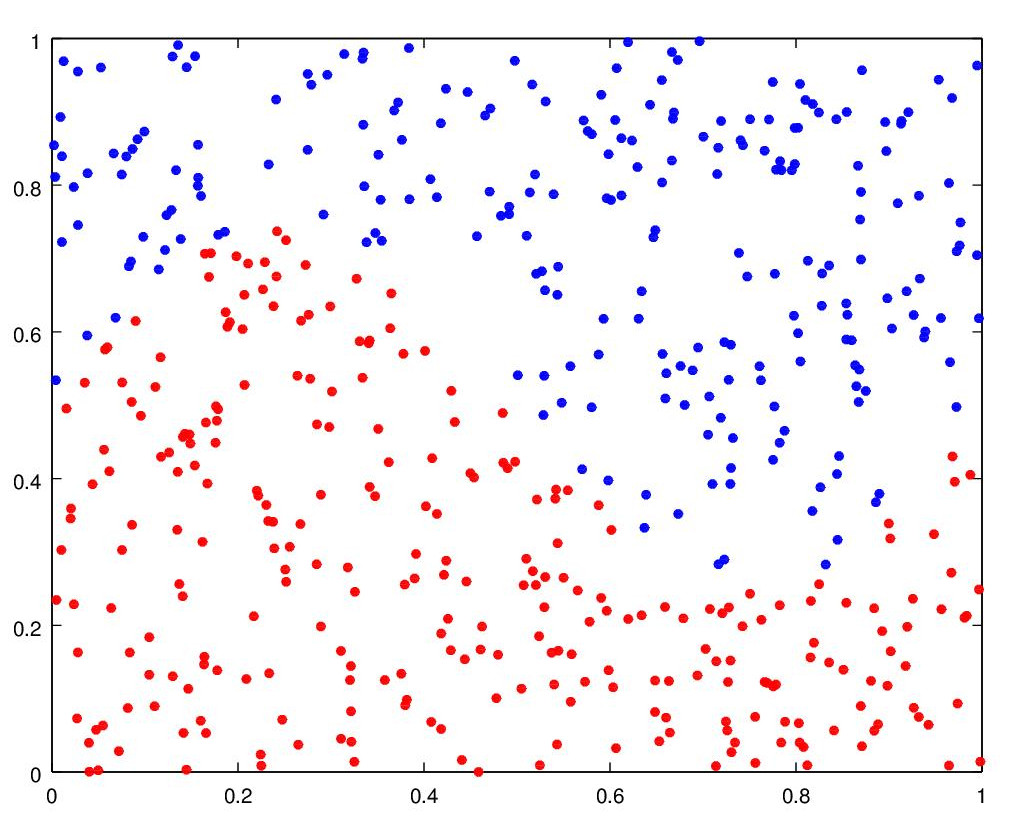
\includegraphics[width=0.8\textwidth]{problem_1}
    \captionsetup{justification=centering,margin=6em}
    \caption{\footnotesize نمایش افراز فضای الگو
$[0, 1] \times [0, 1]$
به دو بخش مثبت(کلاس ۲ -- نقاط آبی) و منفی(کلاس ۱ -- نقاط قرمز) توسط تابع مساله\ ی ۱    
     }
    \label{fig:problem_1}
\end{figure}
\noindent
جدول
\ref{tab:results}
نتایج چندین اجرای الگوریتم بروی مساله\ ی ۱ مقاله می\ باشد.
\begin{latin}
\begin{table}[h]
    \begin{adjustwidth}{-3em}{}
        \begin{tabular}{ | c | c | c | c | c | c | c | c | }
            \cline{5-8}
            \multicolumn{4}{l}{} & \multicolumn{2}{|p{2.5cm}|}{The number of patterns = 40} & \multicolumn{2}{|p{2.5cm}|}{The number of patterns = 100}\\\hline
            Test\# & Shape of fuzzy set & Type of operator & Grade of certainty & Currect & Unclass & Currect & Unclass\\\hline
			1 & Triangular	& Product	& With CF		& 95.53 & 0.0 & 93.24 & 0.0\\\hline
			2 & Trapezoid	& Product	& With CF		& 96.23 & 0.0 & 95.32 & 0.6\\\hline
			3 & Triangular	& Product	& Without CF	    & 94.32 & 0.0 & 93.0 & 0.0\\\hline
			4 & Trapezoid	& Product	& Without CF	    & 69.15 & 31.0 & 63.33 & 36.33\\\hline
			5 & Triangular	& Min		& With CF		& 95.97 & 0.0 & 94.10 & 0\\\hline
			6 & Triangular	& Min		& Without CF 	& 93.45 & 0.0 & 91.0 & 0\\\hline
        \end{tabular}
        \caption{Average rates of correctly classified patterns and unclassified patterns}
        \label{tab:results}
    \end{adjustwidth}
\end{table}
\end{latin}
\newpage
\قسمت{جمع\ بندی و نتیجه\ گیری}
با توجه به نتایج جدول
\ref{tab:results}
مشاهده می\ شود پیاده\ سازی بنده به جز در تست شماره\ ی ۴(تست با تابع عضویت ذوزنقه، اوپراتور ضرب و بدون درجه\ ی اطمینان) در مابقی تست\ ها نتایجی بهتر از نتایج مقاله گرفته است، یک دلیل که چرا ممکن است ظاهرا نتیجه\ ی بهتر حاصل شده است این می\ تواند باشد که این نتایج حاصل از اعمال الگوریتم فقط و فقط روی مساله شماره ۱ مقاله می\ باشد و دیگر مسائل در نظر گرفته نشده است. ولی به قطع میتوان گفت که پیاده\ سازی انجام شده هم\ ارز پیاده\ سازی مقاله می\ باشد. ولی علت اینکه چرا تست شماره\ ی ۴ با اختلاف زیاد هم نسبت به دیگر نتایج حاصل از پیاده\ سازی بنده و هم نسبت به نتایج گزارش شده مقاله کمتر است را نمیدانم، چندین بار کدها را بررسی کردم ولی علت امر برایم آشکار نشد. از آنجایی که کدها بسیار ساخت\ یافته نوشته شده\ اند و هنگام پیاده\ سازی از تکنیک
\lr{DRY}\زیرنویس{\lr{Don't Repeat Yourself}}
پیروی شده است، نمی\ توان گفت شاید الگوریتم نوشته شده دارای اشتباه بوده است؛ چون در این صورت نتایج دیگر تست\ ها نیز خراب می\ شد. به هرحال علت اینکه چرا همه تست\ ها نتایجی بهتر از مقاله دادند و فقط تست شماره ۴ نتیجه\ ای بدتر داده است برایم معما باقی ماند.
\section{مراجع}
\renderref{reference}
\end{document}
